% Lesson 10: shared student/instructor board-supported handout.
% Content: supplied lecture_09(1).tex and lecture_10.tex.
% Structure: converted from the standalone Lesson 10 handout to match the
% wrapper/body layout used by Lessons 01--09.
%
% Source-handling decisions:
% - The narrow-resonance derivation retains the standalone handout's local
%   source approximation and interpretation checkpoints.
% - Solution reveals are supplied only for algebraic blanks and arithmetic
%   table entries directly implied by the public prompt.
% - Qualitative checkpoints remain student annotation space.
% - Editorial/source limitations are documented in instructor_notes.md.

\providecommand{\dd}{\,\mathrm{d}}
\usetikzlibrary{arrows.meta}
\setlength{\abovedisplayskip}{4pt plus 1pt minus 1pt}
\setlength{\belowdisplayskip}{4pt plus 1pt minus 1pt}
\setlength{\abovedisplayshortskip}{3pt plus 1pt}
\setlength{\belowdisplayshortskip}{3pt plus 1pt}
\setlength{\jot}{2pt}
\tcbset{handout base/.append style={before skip=2.5pt,after skip=2.5pt}}

\HandoutSetup
  {NE 630}
  {10}
  {Resonance Absorption}
  {FNRP \S3.4; review Lesson 09}

\begin{document}
\MakeHandoutTitle

\textcolor{KSUDeepPurple}{\textbf{Primary objective.}}
Approximate the epithermal flux spectrum in an infinite, homogeneous
moderator--fuel mixture with resonance absorption.
\par\vspace{5pt}

\begin{handoutcolumns}
\HandoutSection{1}{A Quick Review}

Recall, we're balancing neutrons at an energy $E$ in an infinite, homogeneous
material using the {\it spectrum equation}:
\begin{equation*}
  \overbrace{\Sigma_t(E)\phi(E)}^{\text{all losses from } E} =
    \overbrace{\int_E^{\infty} \frac{\Sigma_s(E'\to E)\phi(E')}{E'} \dd E'}^{\text{gains by scattering}}
    + \overbrace{\chi(E)s_f'''}^{\text{gains from fission}} \, .
\end{equation*}
If we {\it assume} that (1) any neutron above 0.1 MeV scatters immediately to below 0.1 MeV and
(2) neutrons below 0.1 MeV can only scatter elastically and isotropically (in the CM system), then
\begin{equation*}
  \phi(E) \approx
  \begin{cases}
    \displaystyle\frac{\chi(E) s_f'''}{\Sigma_t(E)}  , & E > 0.1\text{ MeV},                  \\
    \displaystyle\frac{s_f'''}{\xi \Sigma_s(E) E},     & 1\text{ eV} < E \le 0.1\text{ MeV} \, .
  \end{cases}
\end{equation*}
If $\Sigma_t(E)$ is constant, then $\phi(E) \propto \chi(E)$ in the fast range, while
$\phi(E) \propto 1/E$ in the epithermal range.

\begin{checkpoint}
What is $s_f'''$?  What is $\xi$?  Why is 0.1 MeV significant?
\RuledLines{3}
\end{checkpoint}

\HandoutSection{2}{Add fuel and absorption}

Let $m$ denote the moderator and $f$ the fuel. Define the in-scatter contribution for $i \in \{m, f\}$ as
$$
 I_i(E)=\int_E^{E/\alpha_i}
 \frac{\Sigma_s^i(E')\phi(E')}{(1-\alpha_i)E'}\dd E'.
$$
The epithermal balance becomes
$$
 \boxed{\Sigma_t(E)\phi(E)=I_m(E)+I_f(E)} \, ,
$$
where $\Sigma_t=\Sigma_s^m+\Sigma_s^f+\Sigma_a^m+\Sigma_a^f$.

\begin{checkpoint}
Why does the left side contain $\Sigma_t$, but the right side contains only scattering cross sections and no source?
\RuledLines{2}

\end{checkpoint}

\switchcolumn
\RaggedRight
\HandoutSection{3}{Resonances and Absorption}

Recall that resonances in the absorption cross section are narrow peaks at specific energies.
Clearly, if a neutron {\it lands} in a resonance it is absorbed, but how likely is it
to actually hit that narrow energy window?  It depends a lot on its last collision.

{\centering
\textbf{Narrow resonance (NR)}\par\vspace{-2pt}
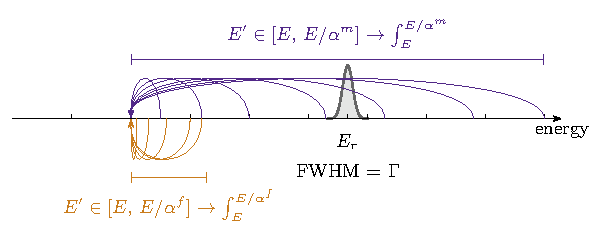
\includegraphics[width=0.98\linewidth]{figures/nr.pdf}\par\smallskip
\textbf{Wide resonance (WR)}\par\vspace{-2pt}
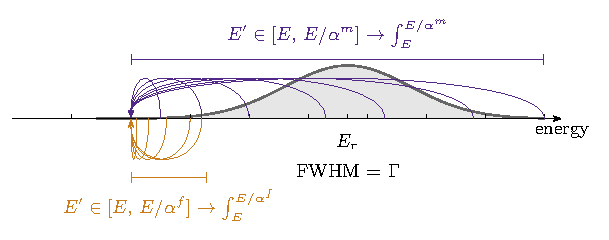
\includegraphics[width=0.98\linewidth]{figures/wr.pdf}\par
}

For a neutron incident near the resonance energy $E \approx E_r$,
$$
 \alpha_i E_r\le E' \le E_r,
 \qquad
 \Delta E_i=(1-\alpha_i)E_r.
$$
Remember that $\Delta E_i$ is the \textbf{maximum allowed loss} in a single collision for nuclide $i$,
but it can be much smaller depending on the scattering angle.

\begin{fixedbox}{Key Assumptions for Narrow Resonance Approximation}
The resonance is narrow on the moderator \emph{and} fuel energy-transfer scales:
$$
 \Delta E_{\mathrm{res}}\ll(1-\alpha_m)E_r,
 \qquad
 \Delta E_{\mathrm{res}}\ll(1-\alpha_f)E_r.
$$
\end{fixedbox}

\begin{checkpoint}
If $E_r=10$ eV and $\Delta E_{\mathrm{res}}=0.50$ eV, compute $\Delta E$ for U-238 and H-1.  Which target clearly fails the NR scale comparison?
\RuledLines{3}
\end{checkpoint}

\end{handoutcolumns}

\newpage
\HandoutSection{4}{Approximate the scattering source}
To evaluate $I_m$ and $I_f$ without first knowing the detailed flux, we assume the following:
\begin{enumerate}
\item Absorption is negligible \emph{between} resonances, so the flux has the shape $C/E'$.
\item $\Sigma^i_s(E) \approx \Sigma_{s,0}^i$ is constant.
\item The resonance is narrow as defined above.
\end{enumerate}
\begin{takeawaybox}[The approximation is made on the right side]
Approximate $\Sigma_s^i(E')\phi(E')$ in $I_i(E)$ by $\Sigma_{s,0}^i C/E'$, but \textbf{retain the energy-dependent total} $\Sigma_t(E)$ on the left.
\end{takeawaybox}

\begin{handoutcolumns}
\HandoutSection{5}{Derive the NR spectrum}
For either scattering nuclide, insert the background approximation from Section 4:
\begin{align*}
 I_i(E)
 &\approx \frac{C\Sigma_{s,0}^i}{1-\alpha_i}
    \int_E^{E/\alpha_i}\frac{\dd E'}{E'^2}\\[3pt]
 &=\frac{C\Sigma_{s,0}^i}{1-\alpha_i}
    \left(\frac{1}{E}-\MathBlank[0.50in]{\alpha_i/E}\right)\\[3pt]
 &=\MathBlank[1.00in]{C\Sigma_{s,0}^i/E}.
\end{align*}
For hydrogen, take $\alpha_i=0$ and integrate to $\infty$; the same result follows.

\begin{boardbox}{Put the two contributions back into balance}
Define $\Sigma_{s,0}=\Sigma_{s,0}^m+\Sigma_{s,0}^f$. Then
$$
 \Sigma_t(E)\phi_{\mathrm{NR}}(E)
 \approx \MathBlank[1.15in]{C\Sigma_{s,0}/E}.
$$
Divide by $\Sigma_t(E)$:
$$
 \boxed{\phi_{\mathrm{NR}}(E)\approx
 \frac{C\Sigma_{s,0}}{\Sigma_t(E)E}}
 \quad\Longrightarrow\quad
 \boxed{\phi_{\mathrm{NR}}\propto\frac{1}{\Sigma_t E}}.
$$
This is the NR result (like FNRP 3.29).
\end{boardbox}

\textbf{Keep the constants straight.} $\Sigma_{s,0}$ is the constant background used in the source approximation, \emph{not} the detailed $\Sigma_s(E)$. The slowing-down supply fixes $C$; this local argument determines the shape.

\begin{checkpoint}[Two limiting checks]
With the same $C$, what happens when:
\begin{enumerate}
\item absorption vanishes and $\Sigma_t=\Sigma_{s,0}$?
\item $\Sigma_t(E_r)$ increases while the approximate scattering-in source stays fixed?
\end{enumerate}
\RuledLines{3}

\end{checkpoint}

\begin{takeawaybox}[When NR Fails]
When the resonance is not narrow for fuel scattering, the replacement of $I_f$ is not justified by this argument. In such cases, the {\it wide resonance} (WR) approximation may be more appropriate.
\end{takeawaybox}

\switchcolumn
\RaggedRight
\HandoutSection{6}{Interpret the flux and reaction rate}
Compare the NR spectrum with the same background $\phi_{\mathrm{bg}}=C/E$:
$$
 \boxed{\frac{\phi_{\mathrm{NR}}(E)}{\phi_{\mathrm{bg}}(E)}
 \approx\frac{\Sigma_{s,0}}{\Sigma_t(E)}}.
$$
Thus a resonance peak in $\Sigma_t$ produces a depression in the flux relative to its $1/E$ background.

\begin{boardbox}{Sketch the consequence}
Sketch $E\phi_{\mathrm{NR}}/C$ for an isolated absorption resonance. The dashed line is the undisturbed $1/E$ spectrum in these coordinates.
\par\smallskip
\centering
\begin{tikzpicture}[x=0.49cm,y=1.55cm,>=Latex]
  \draw[->,thin] (0,0)--(10.8,0) node[right] {$E$};
  \draw[->,thin] (0,0)--(0,1.43) node[above right] {$E\phi/C$};
  \draw[dashed,KSUGray] (0.2,1)--(10.2,1);
  \node[left] at (0,1) {$1$};
  \draw[KSUGray!50,densely dotted] (5.2,0)--(5.2,1.1);
  \node[below] at (5.2,0) {$E_r$};

\end{tikzpicture}
\par\raggedright\scriptsize Schematic prompt; no evaluated nuclear data are implied.
\end{boardbox}

\textbf{A derived interpretation.} A lower flux at the absorption peak reduces absorption relative to using an undisturbed flux there. This is \emph{energy self-shielding}.

\begin{checkpoint}[A flux dip does not mean zero absorption]

Hold fixed the background slowing-down
density $q$ supplying the resonance, in neutrons/cm$^3$-s.
Using $C=q/(\bar{\xi}\Sigma_{s,0})$, we obtain
$$
\phi_{\mathrm{bg}}(E)
=\frac{q}{\bar{\xi}\Sigma_{s,0} E},
\qquad
\phi_{\mathrm{NR}}(E)
\approx\frac{q}{\bar{\xi}\Sigma_t(E)E}.
$$
With $R_a(E)=\Sigma_a(E)\phi_{\mathrm{NR}}(E)$, this gives
$$
\frac{\phi_{\mathrm{NR}}}{\phi_{\mathrm{bg}}}
\approx\frac{1}{1+x},
\qquad
\frac{\bar{\xi} E R_a}{q}
\approx\frac{x}{1+x}.
$$
\renewcommand{\arraystretch}{1.28}
\par\noindent
\begin{tabularx}{\linewidth}
{@{}c>{\centering\arraybackslash}X>{\centering\arraybackslash}X@{}}
\toprule
$x$ & $\phi_{\mathrm{NR}}/\phi_{\mathrm{bg}}$
    & $\bar{\xi} E R_a/q$\\
\midrule
$0$ & $1$ & $0$\\
$1$ & \MathBlank[0.65in]{1/2}
    & \MathBlank[0.65in]{1/2}\\
$9$ & \MathBlank[0.65in]{1/10}
    & \MathBlank[0.65in]{9/10}\\
\bottomrule
\end{tabularx}\par
\smallskip
As $x$ increases at fixed $E$, the flux decreases, but the
absorption rate approaches $q/(\bar{\xi}E)$ rather than zero.
The last column is a scaled rate, not the fraction of source
neutrons absorbed across the resonance.
\end{checkpoint}

\end{handoutcolumns}


\end{document}
